\documentclass[aspectratio=169, 10pt]{beamer}

% ---------- Tema y colores ----------
\usetheme{default}
\usecolortheme{default}
\setbeamertemplate{navigation symbols}{}
\setbeamertemplate{footline}[frame number]
\setbeamertemplate{frametitle continuation}{}

\definecolor{StanfordRed}{RGB}{140,21,21}
\definecolor{StanfordGray}{RGB}{77,77,77}
\definecolor{LightGray}{RGB}{240,240,240}
\definecolor{AccentBlue}{RGB}{0,84,166}
\definecolor{AccentGreen}{RGB}{0,130,100}
\definecolor{UCMBlue}{RGB}{4, 171, 226}
\definecolor{UCMNavy}{RGB}{20, 65, 134}

% Alias de la paleta antigua: las figuras TikZ de esta clase siguen
% usando mitblue/mitgray, que ahora apuntan a los colores UCM.
\definecolor{mitblue}{RGB}{20, 65, 134}
\definecolor{mitgray}{RGB}{169, 169, 169}

\setbeamercolor{frametitle}{fg=white, bg=UCMBlue}
\setbeamercolor{title}{fg=white}
\setbeamercolor{author}{fg=white}
\setbeamercolor{institute}{fg=white!80}
\setbeamercolor{structure}{fg=UCMBlue}
\setbeamercolor{block title}{bg=UCMBlue!15!white, fg=UCMBlue}
\setbeamercolor{block body}{bg=LightGray}
\setbeamercolor{block title alerted}{bg=StanfordRed!15!white, fg=StanfordRed}
\setbeamercolor{block body alerted}{bg=LightGray}
\setbeamercolor{block title example}{bg=AccentGreen!15!white, fg=AccentGreen}
\setbeamercolor{block body example}{bg=LightGray}
\setbeamercolor{alerted text}{fg=UCMBlue}
\setbeamercolor{example text}{fg=UCMBlue}

\setbeamerfont{frametitle}{series=\bfseries, size=\large}
\setbeamerfont{title}{series=\bfseries, size=\LARGE}
\setbeamerfont{block title}{series=\bfseries}

% ---------- Paquetes ----------
\usepackage[utf8]{inputenc}
\usepackage[T1]{fontenc}
\usepackage[provide=*,spanish]{babel}
\usepackage{amsmath, amssymb, bm}
\usepackage{graphicx}
\usepackage{tikz}
\usepackage{pgfplots}
\pgfplotsset{compat=1.18}
\usetikzlibrary{arrows, arrows.meta, shapes, shapes.geometric, positioning,
	fit, calc, matrix, chains, mindmap, decorations.pathreplacing,
	backgrounds, shadows, patterns}
\usepackage{booktabs}
\usepackage{xcolor}
\usepackage{multicol}
\usepackage{tcolorbox}
\tcbuselibrary{skins, breakable}
\usetikzlibrary{circuits.logic.US}

% ---------- Estilos TikZ propios de esta clase ----------
\tikzset{
	neuron/.style={circle, draw, fill=blue!20, minimum size=1.7em, inner sep=0pt},
	input/.style={neuron, fill=green!20},
	output/.style={neuron, fill=red!20},
	hidden/.style={neuron, fill=blue!20},
	bias/.style={neuron, fill=orange!20},
	line/.style={draw, -latex}
}
\pgfmathdeclarefunction{gauss}{2}{%
	\pgfmathparse{1/(#2*sqrt(2*pi))*exp(-((x-#1)^2)/(2*#2^2))}%
}

% ---------- Comandos útiles ----------
\providecommand{\R}{\mathbb{R}}
\providecommand{\E}{\mathbb{E}}
\providecommand{\Var}{\operatorname{Var}}
\providecommand{\relu}{\operatorname{ReLU}}

\newcommand{\formula}[1]{%
	\begin{tcolorbox}[colback=UCMBlue!8, colframe=UCMBlue, arc=4pt,
		boxsep=2pt, left=6pt, right=6pt, top=3pt, bottom=3pt]
		#1
	\end{tcolorbox}
}

% ---------- Portada ----------
\title{\textbf{Optimizaci\'on en Redes Neuronales}}
\subtitle{Descenso de gradiente y regularizaci\'on}
\author{Sergio Hern\'andez, PhD\\ shernandez@ucm.cl}
\institute{
	\begin{tikzpicture}[scale=0.42, every node/.style={transform shape}]
		\foreach \i/\y in {1/0,2/1,3/2}{\node[circle,draw=white,fill=white!20,minimum size=4mm] (i\i) at (0,\y){};}
		\foreach \i/\y in {1/-0.5,2/0.5,3/1.5,4/2.5}{\node[circle,draw=white,fill=white!35,minimum size=4mm] (h\i) at (2,\y){};}
		\foreach \i/\y in {1/0.5,2/1.5}{\node[circle,draw=white,fill=white!50,minimum size=4mm] (o\i) at (4,\y){};}
		\foreach \a in {1,2,3}\foreach \b in {1,2,3,4}{\draw[white,opacity=0.5] (i\a)--(h\b);}
		\foreach \a in {1,2,3,4}\foreach \b in {1,2}{\draw[white,opacity=0.5] (h\a)--(o\b);}
	\end{tikzpicture}
	\\ \textbf{Mag\'ister en Data Science --- Universidad Cat\'olica del Maule}}
\date{}


\begin{document}
% --- Título ---
{
	\setbeamertemplate{background}{
		\begin{tikzpicture}[remember picture, overlay]
			\fill[UCMBlue] (current page.south west) rectangle (current page.north east);
			\fill[UCMBlue!70!black, opacity=0.5]
			(current page.south west) -- ++(0,3) -- ++(18,0) -- cycle;
			\foreach \i in {1,...,40}{
				\fill[white, opacity=0.04]
				({random()*17}, {random()*10}) circle ({random()*0.3});
			}
		\end{tikzpicture}
	}
	\begin{frame}[plain]
		\vspace{1.2cm}
		\titlepage
		\begin{tikzpicture}[remember picture, overlay]
			\node[white, opacity=0.15, font=\fontsize{80}{80}\selectfont]
			at (current page.east) [xshift=-2cm] {$\nabla$};
		\end{tikzpicture}
	\end{frame}
}

\section{Introducci\'on}
% --- Diapositiva 1: Introducción ---
% =================================================================
% SECCIÓN 1: OPTIMIZACIÓN
% =================================================================
\section{Optimización: El Descenso al Mínimo}

% -----------------------------------------------------------------
% DIAPOSITIVA: SUPERFICIE DE ERROR
% -----------------------------------------------------------------
\begin{frame}
	\frametitle{Superficie de Error}
	
	La función de pérdida \(E(\mathbf{\theta})=\sum_i \mathcal L(y_i,\hat y_i)\) define una superficie de error sobre el espacio de todos los posibles parámetros \(\mathbf{\theta}\).
	
	\begin{itemize}
		\item El objetivo de la optimización es encontrar el punto más bajo en esta superficie.
		\item Los algoritmos se basan en el \textbf{gradiente} \(\nabla E(\mathbf{\theta})\), un vector que apunta en la dirección de máximo crecimiento del error. Nos movemos en la dirección opuesta: \(-\nabla E(\mathbf{\theta})\) 
	\end{itemize}
	
	\begin{figure}
		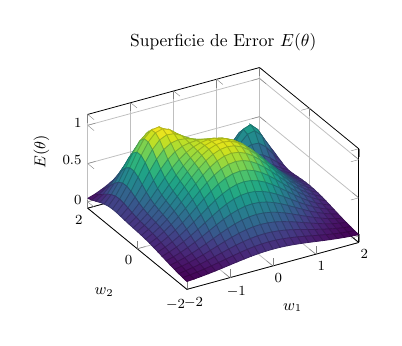
\begin{tikzpicture}[scale=0.7, every node/.style={scale=0.9}]
			\begin{axis}[
				title={Superficie de Error $E(\theta)$},
				xlabel={\(w_1\)},
				ylabel={\(w_2\)},
				view={-30}{45},
				zlabel={$E(\theta)$},
				small,
				grid=major,
				colormap/viridis,
				]
				\addplot3[surf, shader=faceted, domain=-2:2, domain y=-2:2, samples=25]
				{exp(-(x^2+y^2)/2) + 0.5*exp(-((x-1.5)^2+(y-1.5)^2)/0.2) + 0.7*exp(-((x+1)^2+(y-1.2)^2)/0.5)};
				
				% Annotations
				%\node[pin={pin edge={thick, black}, text=black, pin distance=1.5cm, label={[black]225:Mínimo Global}}] at (axis cs: 0,0,1) {};
				%\node[pin={pin edge={thick, black}, text=black, pin distance=1.5cm, label={[black]45:Mínimo Local}}] at (axis cs: -1, -1.2, 0.7) {};
			\end{axis}
		\end{tikzpicture}
		
	\end{figure}
\end{frame}

% -----------------------------------------------------------------
% DIAPOSITIVA: DESAFÍOS DE OPTIMIZACIÓN
% -----------------------------------------------------------------
\begin{frame}
	\frametitle{Optimización en Aprendizaje Profundo}
	

			\textbf{1. Mínimos Locales:} El algoritmo puede converger a un mínimo que no es el global, resultando en un modelo subóptimo. La naturaleza estocástica de SGD (mini-batches) ayuda a escapar.
			
			\vspace{0.5cm}
			
			\textbf{2. Puntos de Silla:} Puntos donde el gradiente es cero, pero no son un mínimo. En dimensiones altas, son \alert{mucho más comunes} que los mínimos locales. En un punto de silla, la matriz Hessiana tiene autovalores positivos y negativos.
			
			\begin{figure}
				\pgfplotsset{width=7cm,compat=1.17} 
					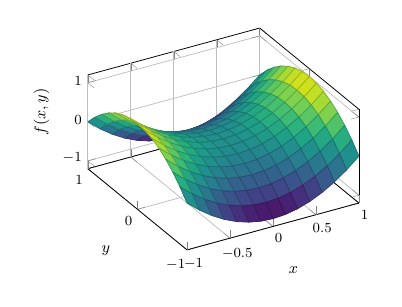
\begin{tikzpicture}[scale=0.7, every node/.style={scale=0.9}]
					\begin{axis}[
						xlabel={\(x\)},
						ylabel={\(y\)},
						view={-30}{45},
						zlabel={$f(x,y)$},
						small,
						grid=major,
						colormap/viridis,
						]
						\addplot3[surf, shader=faceted, domain=-1:1, domain y=-1:1, samples=15]{x^2-y^2};
					\end{axis}
				\end{tikzpicture}
				\caption{\footnotesize Visualización de un punto de silla \(f(x,y)=x^2-y^2\). El gradiente es cero en (0,0), pero no es un mínimo.}
			\end{figure}		
\end{frame}

\begin{frame}
	\frametitle{Optimización en Aprendizaje Profundo}
	
	
		
			\textbf{3. Gradientes que se Desvanecen (Vanishing Gradients):} En redes profundas, los gradientes pueden volverse extremadamente pequeños, deteniendo el aprendizaje.
			\begin{itemize}
				\item \small Causa: Multiplicación de números de-normalizados (underflow) en la regla de la cadena. Activaciones como la sigmoide o tanh son propensas a esto.
			\end{itemize}
			
			\vspace{0.5cm}
			
			\textbf{4. Gradientes que Explotan (Exploding Gradients):} los gradientes crecen exponencialmente, causando inestabilidad.
			\begin{itemize}
				\item \small Causa: Multiplicación de números grandes (overflow).
			\end{itemize}
			
			\vfill
			\begin{block}{Soluciones}
				Técnicas como \textbf{activaciones ReLU}, \textbf{Batch Normalization} y \textbf{Conexiones Residuales}  fueron creadas para mitigar estos problemas.
			\end{block}
\end{frame}

\begin{frame}
	\frametitle{Normalización de Datos}
	
		\begin{block}{Normalización de Datos}
		La normalización de datos es una técnica de pre-procesamiento que se aplica sobre los datos de entrada para asegurar que la superficie de error tenga la misma curvatura en cada una de las dimensiones.
	\end{block}
	
\begin{figure}[h!]
\centering
\begin{tabular}{cc}
	% Left Plot: Gradient descent without scaling
	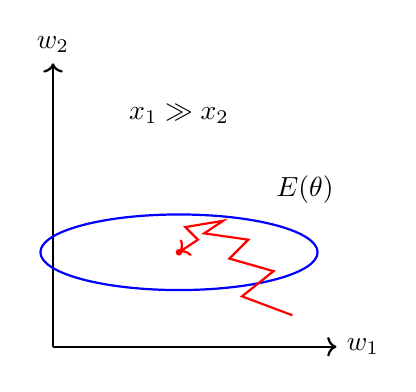
\begin{tikzpicture}[scale=0.8]
		% Title in a green box
		%\node (title1) at (2, 4.7) [draw=green, thick, inner sep=3pt, text width=4cm, align=center] {Gradient descent \\ without scaling};
		
		% Text indicating large feature range difference
		\node at (2, 3.7) {$x_1 \gg x_2$};
		
		% Axes with labels
		\draw[->, thick] (0,0) -- (4.5,0) node[right] {$w_1$};
		\draw[->, thick] (0,0) -- (0,4.5) node[above] {$w_2$};
		
		% Elliptical contour lines (cost function J(w))
		% Center of ellipses, representing the minimum of J(w)
		\coordinate (center1) at (2, 1.5); % Position of the minimum
		
		% Outermost ellipse (thick blue line)
		%\node[ellipse,draw] (e) at (center1) {};
		\draw[blue, thick] (center1) ellipse (2.2cm and 0.6cm); % x-radius and y-radius for elongation
		% Inner ellipses, scaled down
		%\foreach \k in {0.1, 0.2, ..., 0.9} { % Loop to draw multiple concentric ellipses
		%	\draw[blue] (center1) ellipse (2.2cm * \k and 0.6cm * \k);
		%}
		
		% Label for the cost function
		\node at (4.0, 2.5) {$E(\theta)$};
		
		% Gradient descent path (zigzag, slow convergence)
		% Mark the minimum point with a red dot
		\fill[red] (center1) circle (1.5pt); 
		% Draw the path with multiple segments, showing oscillation
		\draw[red, thick, ->] (3.8, 0.5) -- (3.0, 0.8) -- (3.5, 1.2) -- (2.8, 1.4) -- (3.1, 1.7) -- (2.4, 1.8) -- (2.7, 2.0) -- (2.1, 1.9) -- (2.3, 1.7) -- (2.0, 1.5);
		
	\end{tikzpicture}
	& % Separator for tabular columns
	% Right Plot: Gradient descent after scaling variables
	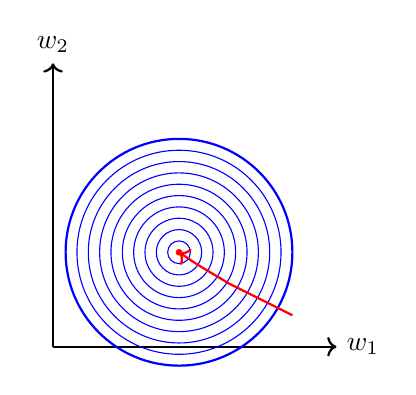
\begin{tikzpicture}[scale=0.8]
		% Title in a green box
	%	\node (title2) at (2, 4.7) [draw=green, thick, inner sep=3pt, text width=4cm, align=center] {Gradient descent \\ after scaling variables};
		
		% Text indicating scaled feature ranges
		%\node at (2, 3.7) {$0 \le x_1 \le 1$};
		%\node at (2, 3.3) {$0 \le x_2 \le 1$};
		
		% Axes with labels
		\draw[->, thick] (0,0) -- (4.5,0) node[right] {$w_1$};
		\draw[->, thick] (0,0) -- (0,4.5) node[above] {$w_2$};
		
		% Circular contour lines (cost function J(w))
		% Center of circles, representing the minimum of J(w)
		\coordinate (center2) at (2, 1.5); % Position of the minimum
		
		% Outermost circle (thick blue line)
		\draw[blue, thick] (center2) circle (1.8); % Radius for circular contours
		% Inner circles, scaled down
		\foreach \k in {0.1, 0.2, ..., 0.9} { % Loop to draw multiple concentric circles
			\draw[blue] (center2) circle (1.8 * \k);
		}
		
		% Label for the cost function
		%\node at (4.0, 2.5) {$E(\theta)$};
		
		% Gradient descent path (direct, fast convergence)
		% Mark the minimum point with a red dot
		\fill[red] (center2) circle (1.5pt); 
		% Draw the path with a few direct segments
		\draw[red, thick, ->] (3.8, 0.5) -- (2.8, 1.0) -- (2.3, 1.3) -- (2.0, 1.5);
		
	\end{tikzpicture}
\end{tabular}
\end{figure}
\end{frame}

\begin{frame}
	\frametitle{Normalización de Lotes}
	
	\begin{block}{Batch Normalization (\textbf{BatchNorm})}
	Normaliza las pre-activaciones dentro de cada capa para cada mini-lote de datos. Específicamente, para cada unidad oculta $i$, calcula la media y la varianza de sus pre-activaciones $x_{in}[i]$ a través de los ejemplos en el mini-lote actual y las utiliza para estandarizar los valores a una media de cero y una varianza unitaria
\end{block}
	\[
		x_{out}[i]=\gamma \frac{x_{in}[i] - \mathbb E \bigr [x_{in} \left[i \right] \bigr] }{\sqrt{\operatorname{Var \bigr[ x_{in}[i]\bigr]}}}+\beta
	\]
	Donde $\gamma$ y $\beta$ son parámetros entrenables.
 \end{frame}

\begin{frame}
	\frametitle{Normalización de Capas }
	
	\begin{block}{Layer Normalization (\textbf{LayerNorm})}
	Existen otros tipos de normalización por capas. Por ejemplo, si calculamos la media $\mu=\frac{1}{d}\sum_i^d x_{in} \left[i \right]$ y varianza de la capa $\sigma^2=\frac{1}{d}\sum_i^d (x_{in} \left[i \right] - \mu)^2$. A diferencia de \texttt{BatchNorm}, la media y varianza se calculan sobre los elementos $x_{in}[i]$.
	\end{block}
%		\begin{align*}
%		x_{out}[i]=\gamma \frac{x_{in}[i] - \mu }{\sigma}+\beta
%	\end{align*}
\begin{figure}[h!]
\centering
\begin{tabular}{cc}
		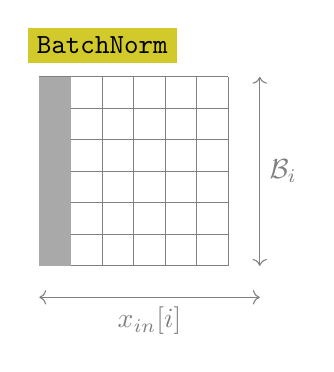
\begin{tikzpicture}[scale=0.4]
		\draw[line width=5pt] (2,7)  node[fill=yellow!80!black] (b) {\texttt{BatchNorm}};
		\draw[step=1cm,gray] (0,0) grid (6,6);
		\fill[mitgray] (0,0) rectangle (1,6);
		\draw[<->,gray]  (7,6) -- (7,0)  node [midway,right,draw=none] {$\mathcal B_i$};
		\draw[<->,gray]  (0,-1) -- (7,-1) node [midway,below,draw=none] {$x_{in} [i]$};
		\end{tikzpicture}
	&
		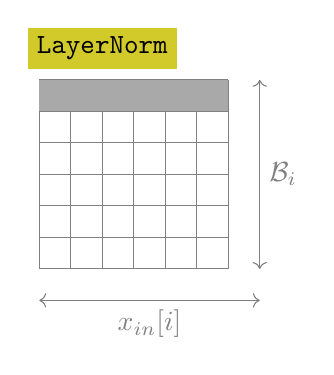
\begin{tikzpicture}[scale=0.4]
		\draw[line width=5pt] (2,7)  node[fill=yellow!80!black] (b) {\texttt{LayerNorm}};
		\draw[step=1cm,gray] (0,0) grid (6,6);
		\fill[mitgray] (0,6) rectangle (6,5);
		\draw[<->,gray]  (7,6) -- (7,0)  node [midway,right,draw=none] {$\mathcal B_i$};
		\draw[<->,gray]  (0,-1) -- (7,-1) node [midway,below,draw=none] {$x_{in} [i]$};
		\end{tikzpicture}
\end{tabular}
\end{figure}
	
\end{frame}
% -----------------------------------------------------------------
% DIAPOSITIVA: ALGORITMOS GD
% -----------------------------------------------------------------
\begin{frame}
	\frametitle{Algoritmos de Descenso de Gradiente (GD)}
	
	\begin{columns}[t]
		\begin{column}{.5\textwidth}
			\begin{block}{Batch GD}
				Calcula el gradiente usando \textbf{todo} el dataset.
				\begin{itemize}
					\item[-] Preciso pero computacionalmente inviable para datasets grandes.
				\end{itemize}
			\end{block}
		\end{column}
		\begin{column}{.5\textwidth}
			\begin{block}{Stochastic GD (SGD)}
				Calcula el gradiente usando \textbf{un solo} dato a la vez.
				\begin{itemize}
					\item[+] Rápido, eficiente y el ruido ayuda a escapar de mínimos locales.
					\item[-] Actualizaciones muy ruidosas.
				\end{itemize}
			\end{block}
		\end{column}
		
	\end{columns}
	\begin{alertblock}{Stochastic GD (SGD)}
	\begin{align*}
		\mathbf{\theta}^{k+1}&\leftarrow \mathbf{\theta}^{k}-\eta \nabla E(\mathbf{\theta}^{k})
	\end{align*}
	\end{alertblock}
\end{frame}

\begin{frame}
	\frametitle{Descenso de Gradiente Estocástico (SGD)}
	
	\begin{columns}[t]
		\begin{column}{.5\textwidth}
			\begin{figure}[h!]
				\centering
				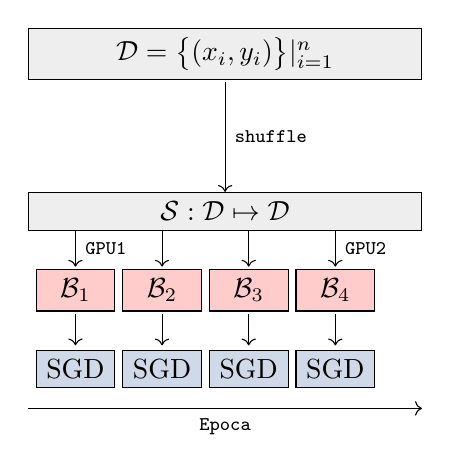
\begin{tikzpicture}[scale=1.0]
				\draw (3,3)     node[minimum width=5cm,draw,fill=mitgray!20] {$\mathcal D=\bigl\{(x_i,y_i)\bigr\}\vert_{i=1}^n$};
				
				\draw (3,1)     node[minimum width=5cm,draw,fill=mitgray!20] {$\mathcal S:\mathcal D \mapsto \mathcal D$};
				
				\node foreach \x in {1,...,4}
				[draw,fill=red!20,minimum width=1cm] at (\x*1.1,0) {$\mathcal B_{\x}$};
				
				\node foreach \x in {1,...,4}
				[draw,minimum width=1cm,fill=mitblue!20] at (\x*1.1,-1) {SGD};
				
				%\node foreach \x in {1,...,4}
				\draw[->]        (3,3-0.35)   -- (3,1+0.25) node [midway,right,draw=none,font=\scriptsize] {\texttt{shuffle}};
				
				\draw[->]        (1.1,-0.3)   -- (1.1,-0.7);
				\draw[->]        (2.2,-0.3)   -- (2.2,-0.7);
				\draw[->]        (3.3,-0.3)   -- (3.3,-0.7);
				\draw[->]        (4.4,-0.3)   -- (4.4,-0.7);
				
				\draw[->]        (1.1,1.0-0.25)   -- (1.1,0.0+0.3) node [midway,right,draw=none,font=\scriptsize] {\texttt{GPU1}};
				\draw[->]        (2.2,1.0-0.25)   -- (2.2,0.0+0.3);
				\draw[->]        (3.3,1.0-0.25)   -- (3.3,0.0+0.3);
				\draw[->]        (4.4,1.0-0.25)   -- (4.4,0.0+0.3) node [midway,right,draw=none,font=\scriptsize] {\texttt{GPU2}};
				
				\draw[->]        (0.5,-1.5)   -- (5.5,-1.5) node [midway,below,draw=none,font=\scriptsize] {\texttt{Epoca}};
			\end{tikzpicture}
		\end{figure}
		\end{column}

		\begin{column}{.5\textwidth}
		\begin{block}{Mini-batch SGD}
			Calcula el gradiente $\nabla_{\mathcal B_k} E(\mathbf{\theta}^{k})$ sobre un \textbf{pequeño lote} $|\mathcal B_k|<<n$ (mini-batch) de datos.
			
			\begin{itemize}
				\item[+] Reduce el ruido y aprovecha la computación paralela (multi-GPU).
				\item[+] Para modelos grandes, es posible combinar paralelismo de datos y paralelismo de modelos.
			\end{itemize}
		\end{block}
	\end{column}
		\end{columns}
\end{frame}

\begin{frame}
	\frametitle{Algoritmos de Descenso de Gradiente (GD)}
	

	
	\begin{block}{\textbf{Momentum}}
		\begin{itemize}
			\item Es una forma de solucionar el problema de valores propios de la matriz Hessiana es agregar un término de \textbf{momento}. Ayuda a acelerar en direcciones de baja curvatura y amortiguar oscilaciones .
			\[
			\begin{split}\begin{aligned}
					\mathbf{v}^{k} &\leftarrow \beta \mathbf{v}^{k-1} - \eta  E(\mathbf{\theta}^{k}), \\
					\mathbf{\theta}^{k+1}&\leftarrow \mathbf{\theta}^{k}+\mathbf{v}^{k}
			\end{aligned}\end{split}
		\]
			\item \textbf{Nesterov:}  Modifica el algoritmo de \textbf{momento}, utilizando el gradiente en una posición futura proyectada.
			\[
			\mathbf{v}^{k+1} \leftarrow \beta \mathbf{v}^{k-1} - \eta E(\mathbf{\theta}^{k}+\beta \mathbf{v}^{k})
			\]
		\end{itemize}
	\end{block}
	

\end{frame}

\begin{frame}
	\frametitle{Algoritmos de Descenso de Gradiente (GD)}

	
	\begin{figure}
		\pgfmathsetseed{1}
		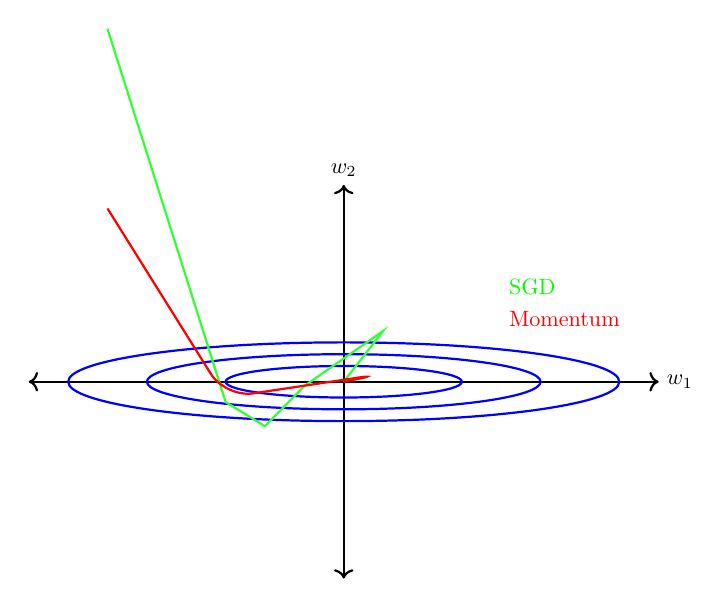
\begin{tikzpicture}[scale=1.0, every node/.style={scale=0.8}]
			\draw[<->,thick] (-4,0) -- (4,0) node[right] {$w_1$};
			\draw[<->,thick] (0,-2.5) -- (0,2.5) node[above] {$w_2$};
			\draw[blue,thick] (0,0) ellipse (3.5cm and 0.5cm);
			\draw[blue,thick] (0,0) ellipse (2.5cm and 0.35cm);
			\draw[blue,thick] (0,0) ellipse (1.5cm and 0.2cm);
			%\node at (0,0) {$\mathbf{w}^*$};
			
			% GD path
			\draw[green!80, thick] (-3,rand*2.2*10) -- (-1.5, rand*-0.2*10) -- (-1.0, rand*-1.2) -- (-0.5, rand*-0.2) -- (0.5, rand*0.1*10) -- (0,0);
			%\node[blue, right] at (1,1.5) {SGD};
			
			% Momentum path
			\draw[red, thick, rounded corners=10pt] (-3,2.2) -- (-1.5, -0.2) -- (0.5, 0.1) -- (0,0);
			\node[green, right] at (2,1.2) {SGD};
			\node[red, right] at (2,0.8) {Momentum};
		\end{tikzpicture}
		\caption{Y. Nesterov, A Method of Solving
			a Convex Programming Problem
			with Convergence Rate O(1/k2 ),
			Soviet Mathematics Doklady, vol. 27,
			no. 2, pp. 543–547, 1983.}
	\end{figure}
\end{frame}

% =================================================================
% SECCIÓN 2: REGULARIZACIÓN
% =================================================================
\section{Regularización}

% -----------------------------------------------------------------
% DIAPOSITIVA: OVERFITTING E INDUCTIVE BIAS
% -----------------------------------------------------------------
\begin{frame}
	\frametitle{Sobreajuste}
	
	\textbf{Problema Inverso:} Dado un conjunto finito de datos, existen infinitos modelos que podrían haberlos generado. ¿Cómo elegimos el correcto?
	
	\begin{figure}
		 \pgfplotsset{width=8cm,compat=1.18}
		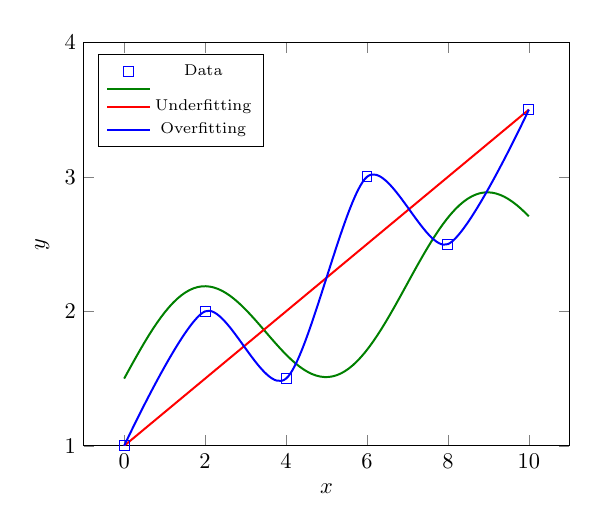
\begin{tikzpicture}[scale=0.9, every node/.style={scale=0.9}]
			\begin{axis}[
				xmin=-1, xmax=11, ymin=1, ymax=4,
				xlabel={\(x\)}, ylabel={\(y\)},
				legend pos=north west,
				]
%				\addplot[only marks, mark=*, blue] table {
%					0 1
%					2 2
%					4 1.5
%					6 3
%					8 2.5
%					10 3.5
%				};
				\addplot[
				only marks,
				color=blue,
				mark=square,
				]
				coordinates {
					(0,1)(2,2)(4,1.5)(6,3)(8,2.5)(10,3.5)
				};
				\addlegendentry{\scriptsize Data}
				\addplot[green!50!black, thick, domain=0:10, samples=100,thick] {1.5 + 0.5*sin(deg(x*0.9)) + 0.1*x};
				\addlegendentry{}
				
				\addplot[red, thick, domain=0:10, samples=100] {0.25*x + 1};
				\addlegendentry{\scriptsize Underfitting}
				

				\addplot[blue, thick, domain=0:10, samples=200, smooth] coordinates {(0,1) (2,2) (4,1.5) (6,3) (8,2.5) (10,3.5)};
				\addlegendentry{\scriptsize Overfitting}
			\end{axis}
		\end{tikzpicture}

	\end{figure}
	
\end{frame}

\begin{frame}
	\frametitle{Sesgo y Varianza}
	
	
	\begin{figure}
		\pgfplotsset{width=8cm,compat=1.18}
		\tikzset{
			target/.style={
				draw=none,
				fill=mitgray!30,
				circle,
				minimum size=5cm
			},
			ring/.style={
				draw=white,
				ultra thick,
				circle
			}
		}
		\begin{tikzpicture}[scale=0.7]
			
			% --- Primera diana: Alto sesgo, baja varianza ---
			\begin{scope}[shift={(-6,0)}]
				% Fondo
				\node[target] at (0,0) {};
				% Anillos
				\foreach \r in {1,2,3}
				\draw[ring] (0,0) circle (\r cm);
				% Centro
				\fill[white] (0,0) circle (0.5cm);
				
				% Puntos (lejos del centro, agrupados)
				\foreach \pos in {(-2.2,0.2),(-2.4,-0.2),(-2.3,0.4),(-2.1,-0.3)}
				\fill[black] \pos circle (5pt);
				
				\node at (0,-3.8) {\textbf{Alto Sesgo, Baja Varianza}};
			\end{scope}
			
			% --- Segunda diana: Bajo sesgo, alta varianza ---
			\begin{scope}[shift={(3,0)}]
				% Fondo
				\node[target] at (0,0) {};
				% Anillos
				\foreach \r in {1,2,3}
				\draw[ring] (0,0) circle (\r cm);
				% Centro
				\fill[white] (0,0) circle (0.5cm);
				
				% Puntos (cerca del centro pero dispersos)
				\foreach \pos in {(0.3,0.4),(1.2,-0.6),(-0.8,0.9),(0.7,-1.1)}
				\fill[black] \pos circle (5pt);
				
				\node at (0,-3.8) {\textbf{Bajo Sesgo, Alta Varianza}};
			\end{scope}
			
		\end{tikzpicture}
	\end{figure}
\end{frame}

\begin{frame}
	\frametitle{Sesgo y Varianza}
	
	
	\begin{figure}
		\pgfplotsset{width=8cm,compat=1.18}
		\tikzset{
			target/.style={
				draw=none,
				fill=mitgray!30,
				circle,
				minimum size=5cm
			},
			ring/.style={
				draw=white,
				ultra thick,
				circle
			}
		}
		\begin{tikzpicture}[scale=0.7]
			
			
			% --- Caso Ideal: Bajo Sesgo, Baja Varianza ---
			\begin{scope}[shift={(-6,0)}]
				\node[target] at (0,0) {};
				\foreach \r in {1,2,3}
				\draw[ring] (0,0) circle (\r cm);
				\fill[white] (0,0) circle (0.5cm);
				
				% Puntos muy cerca del centro
				\foreach \pos in {(0.1,0.1),(0.2,-0.1),(-0.1,0.2),(0.05,-0.05)}
				\fill[black] \pos circle (5pt);
				
				\node at (0,-3.8) {\textbf{Bajo Sesgo, Baja Varianza (Ideal)}};
			\end{scope}
			
			% --- Alto Sesgo, Alta Varianza ---
			\begin{scope}[shift={(2,0)}]
				\node[target] at (0,0) {};
				\foreach \r in {1,2,3}
				\draw[ring] (0,0) circle (\r cm);
				\fill[white] (0,0) circle (0.5cm);
				
				% Puntos dispersos y lejos del centro
				\foreach \pos in {(-2.2,1.5),(-1.5,-2.3),(-2.6,-0.5),(-1.8,2.0)}
				\fill[black] \pos circle (5pt);
				
				\node at (0,-3.8) {\textbf{Alto Sesgo, Alta Varianza}};
			\end{scope}
			
		\end{tikzpicture}
	\end{figure}
\end{frame}

\begin{frame}
	\frametitle{Sesgo Inductivo}
	
	\textbf{Problema Inverso:} Dado un conjunto finito de datos, existen infinitos modelos que podrían haberlos generado. ¿Cómo elegimos el correcto?
	

	\begin{block}{Sesgo Inductivo (Inductive Bias)}
		Para generalizar, necesitamos introducir \textbf{suposiciones} o \textbf{conocimiento previo} sobre la naturaleza de la solución. Esto se llama \textit{sesgo inductivo}.
		\begin{itemize}
			\item \textbf{Teorema de No Free Lunch (Wolpert, 1996) :} Ningún algoritmo es el mejor para todos los problemas. El éxito depende de que el sesgo inductivo del algoritmo coincida con el problema.
			\item La regularización es una forma de introducir un sesgo inductivo explícito.
		\end{itemize}
	\end{block}
\end{frame}




% -----------------------------------------------------------------
% DIAPOSITIVA: TÉCNICAS DE REGULARIZACIÓN
% -----------------------------------------------------------------
\begin{frame}
	\frametitle{Técnicas de Regularización Explícita}
	
	\begin{columns}[T]
		\begin{column}{.48\textwidth}
			\begin{block}{Weight Decay (Regularización L2)}
				Añade un término de penalización a la pérdida: \( E(\theta) + \lambda || \theta||_2 \)
				\begin{itemize}
					\item[-] \textbf{Sesgo inductivo:} Prefiere funciones "más suaves" (con pesos pequeños)
					\item[-] Reduce la varianza del modelo a costa de un pequeño aumento en el sesgo
				\end{itemize}
			\end{block}
		\end{column}
			%\vspace{0.5cm}
			\begin{column}{.48\textwidth}
			\begin{block}{Data Augmentation}
				Aumenta artificialmente el dataset creando versiones transformadas de los datos (rotaciones, recortes, etc.).
				\begin{itemize}
					\item[-] \textbf{Sesgo inductivo:} Enseña explícitamente al modelo a ser invariante a estas transformaciones .
					\item[-] Extremadamente efectivo y fácil de implementar, especialmente para imágenes.
				\end{itemize}
			\end{block}
		\end{column}
		
	
	\end{columns}
\end{frame}

\begin{frame}
	\frametitle{Técnicas de Regularización Explícita}
	
	\begin{columns}[T]
		\begin{column}{.48\textwidth}
		
			\begin{block}{Dropout}
				Durante el entrenamiento, "apaga" neuronas aleatoriamente con una probabilidad \(p\).
				\begin{itemize}
					\item[-] Previene la co-adaptación compleja entre neuronas.
					\item[-] Es una forma eficiente de promediar un número exponencial de redes neuronales distintas (ensemble) .
				\end{itemize}
			\end{block}
		\end{column}
		
		\begin{column}{.48\textwidth}
	
		
			\begin{block}{Early Stopping}
				Monitoriza el error en un set de validación y detiene el entrenamiento cuando este error deja de mejorar.
				\begin{itemize}
					\item[-] La forma más simple de regularización.
					\item[-] Controla la complejidad efectiva del modelo, que aumenta con las épocas de entrenamiento.
				\end{itemize}
			\end{block}
		\end{column}
	\end{columns}
\end{frame}

% -----------------------------------------------------------------
% DIAPOSITIVA: CONCLUSIONES
% -----------------------------------------------------------------
\begin{frame}
	\frametitle{Conclusiones}
	
	\begin{itemize}
		\item \textbf{Descenso del Gradiente} es algoritmo para encontrar un mínimo en la función de pérdida. El \textbf{momento} ayuda a controlar el efecto de los puntos silla.
		
		\item \textbf{La regularización} es una técnica para asegurar que ese mínimo corresponda a un modelo que generaliza. Se basa en el principio fundamental del \textit{sesgo inductivo}.
		
		\item Las innovaciones modernas como \textbf{BatchNorm} y \textbf{LayerNorm} son poderosas porque mejoran tanto la optimización (haciendo el entrenamiento más fácil y rápido) como la regularización (llevando a mejores modelos).
		
		
	\end{itemize}
	
	
\end{frame}

	
\end{document}